\section{Turing Testi}
İngiliz matematikçi ve bilgisayar bilimcisi Alan Turing tarafından 1950 yılında ortaya atılmıştır. Turing testi, yapay zekanın insan zekasına benzer bir seviyeye ulaşıp ulaşmadığını değerlendirmek için kullanılan bir testtir. Bilgisayarın insan dili kadar anlamlı yanıtlar vermesinin mümkün olup olmadığını araştırır. Bir tür sohbet testidir. Savcı, İnsan ve Bilgisayar olmak üzere 3 oyuncudan oluşur. Turing testinde bilgisayarın "düşünen" bir programla donatıldığı varsayılmaktadır. Temel amacı savcının, bilgisayar ve insanın vereceği cevapların kimden geldiğini tespit edebilmesidir. Eğer savcı insanı bilgisayardan ayırabilirse insan kazanmış olur. Fakat bir bilgisayar verilen sorulardaki anahtar kelimeleri bulup programdan o soruların cevaplarını getirdiği için burda bir "anlama" söz konusu değildi. Turing'in bu testte amacı, zekanın modellenmesinin mümkünlüğünü tartışmaktı.

\begin{figure}[h]
    \centering
    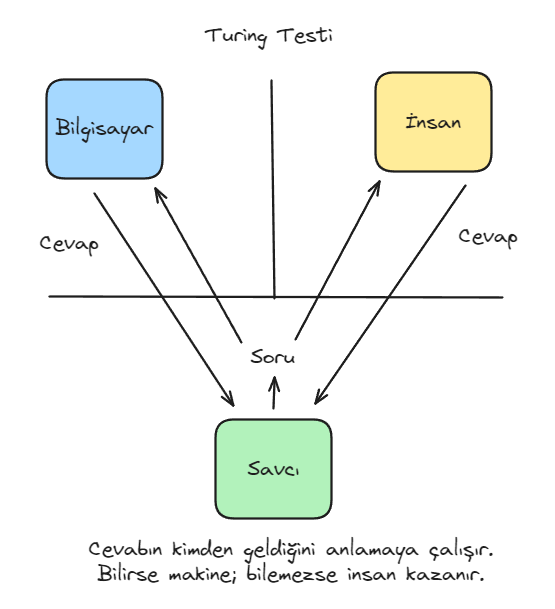
\includegraphics[width=0.8\textwidth]{images/turing_test.png}
    \caption{Turing testi.}
    \label{fig:enter-label}
\end{figure}

\newpage